\section{Problem statement}

\begin{frame}{Problem statement}
    \begin{itemize}
          \item {
            Prevailing neural network architectures are implemented using several hidden layers, with each one consisting of thousands to millions of neurons in order to generalize well on diverse inputs. 
          }
          \item {Can you imagine how many parameters need to be trained for every iterations?
          }
  \end{itemize}
 
  
\begin{figure}[!tbp]
  %\centering
  \begin{minipage}[b]{0.4\textwidth}
    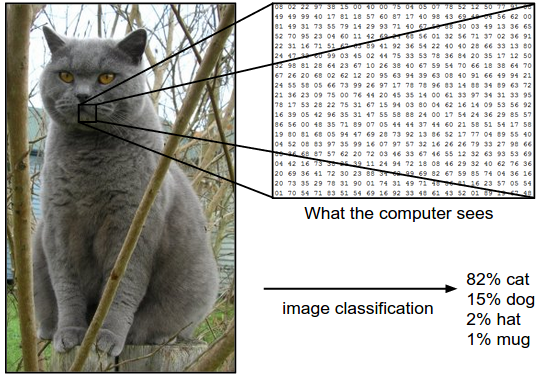
\includegraphics[width=1.6in]{classify.png}
  \end{minipage}
  %\hfill
  \begin{minipage}[b]{0.4\textwidth}
    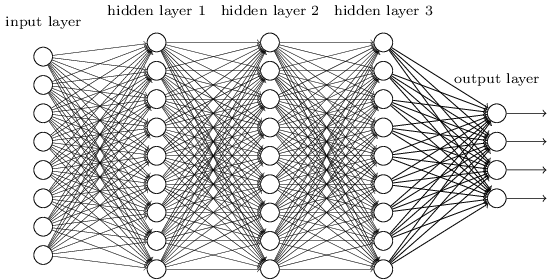
\includegraphics[width=2.4in]{many_nn.png}
  \end{minipage}
\end{figure}

\end{frame}


\begin{frame}{Problem statement(contd.)}
	\begin{itemize}
	\item {Gradient Descent is the most commonly used optimization algorithm used to train neural networks in supervised settings.}
	\item {Having the gradient as a sum of partial gradients with respect to individual training examples opens up the possibility of parallelizing the gradient computation efficiently.}

	\end{itemize}

\end{frame}